\section{A BUSCA POR ANIMAIS PERDIDOS: DIVULGAÇÃO, COLABORAÇÃO E ORGANIZAÇÃO DAS INFORMAÇÕES}

A presença de animais de estimação é expressiva na sociedade brasileira. Em 2019, a Pesquisa Nacional de Saúde (PNS) registrou que 46,1\% dos domicílios particulares permanentes do país possuíam pelo menos um cachorro (33,8 milhões de lares) e 19,3\% possuíam ao menos um gato (14,1 milhões de lares) (IBGE, 2020). No entanto, o convívio com animais domésticos é frequentemente acompanhado pelo risco de perdas acidentais: estudos internacionais apontam que ao menos 15\% dos tutores passam pela experiência de perder seu animal de estimação em um período de cinco anos (Weiss; Slater; Lord, 2012).

A probabilidade de recuperação com vida está diretamente associada à agilidade temporal e à mobilização nos momentos imediatos após a fuga. Ao investigarem a trajetória e os desfechos de animais desaparecidos, Huang et al. (2018) demonstraram a existência de uma janela crítica de buscas, ilustrada na Figura~\ref{fig:curva_recuperacao_tempo}.

\begin{figure}[H]
    \centering
    \caption{Percentual acumulado de gatos perdidos encontrados vivos em função dos dias decorridos: (a) primeiro ano e (b) primeiros trinta dias}
    \label{fig:curva_recuperacao_tempo}
    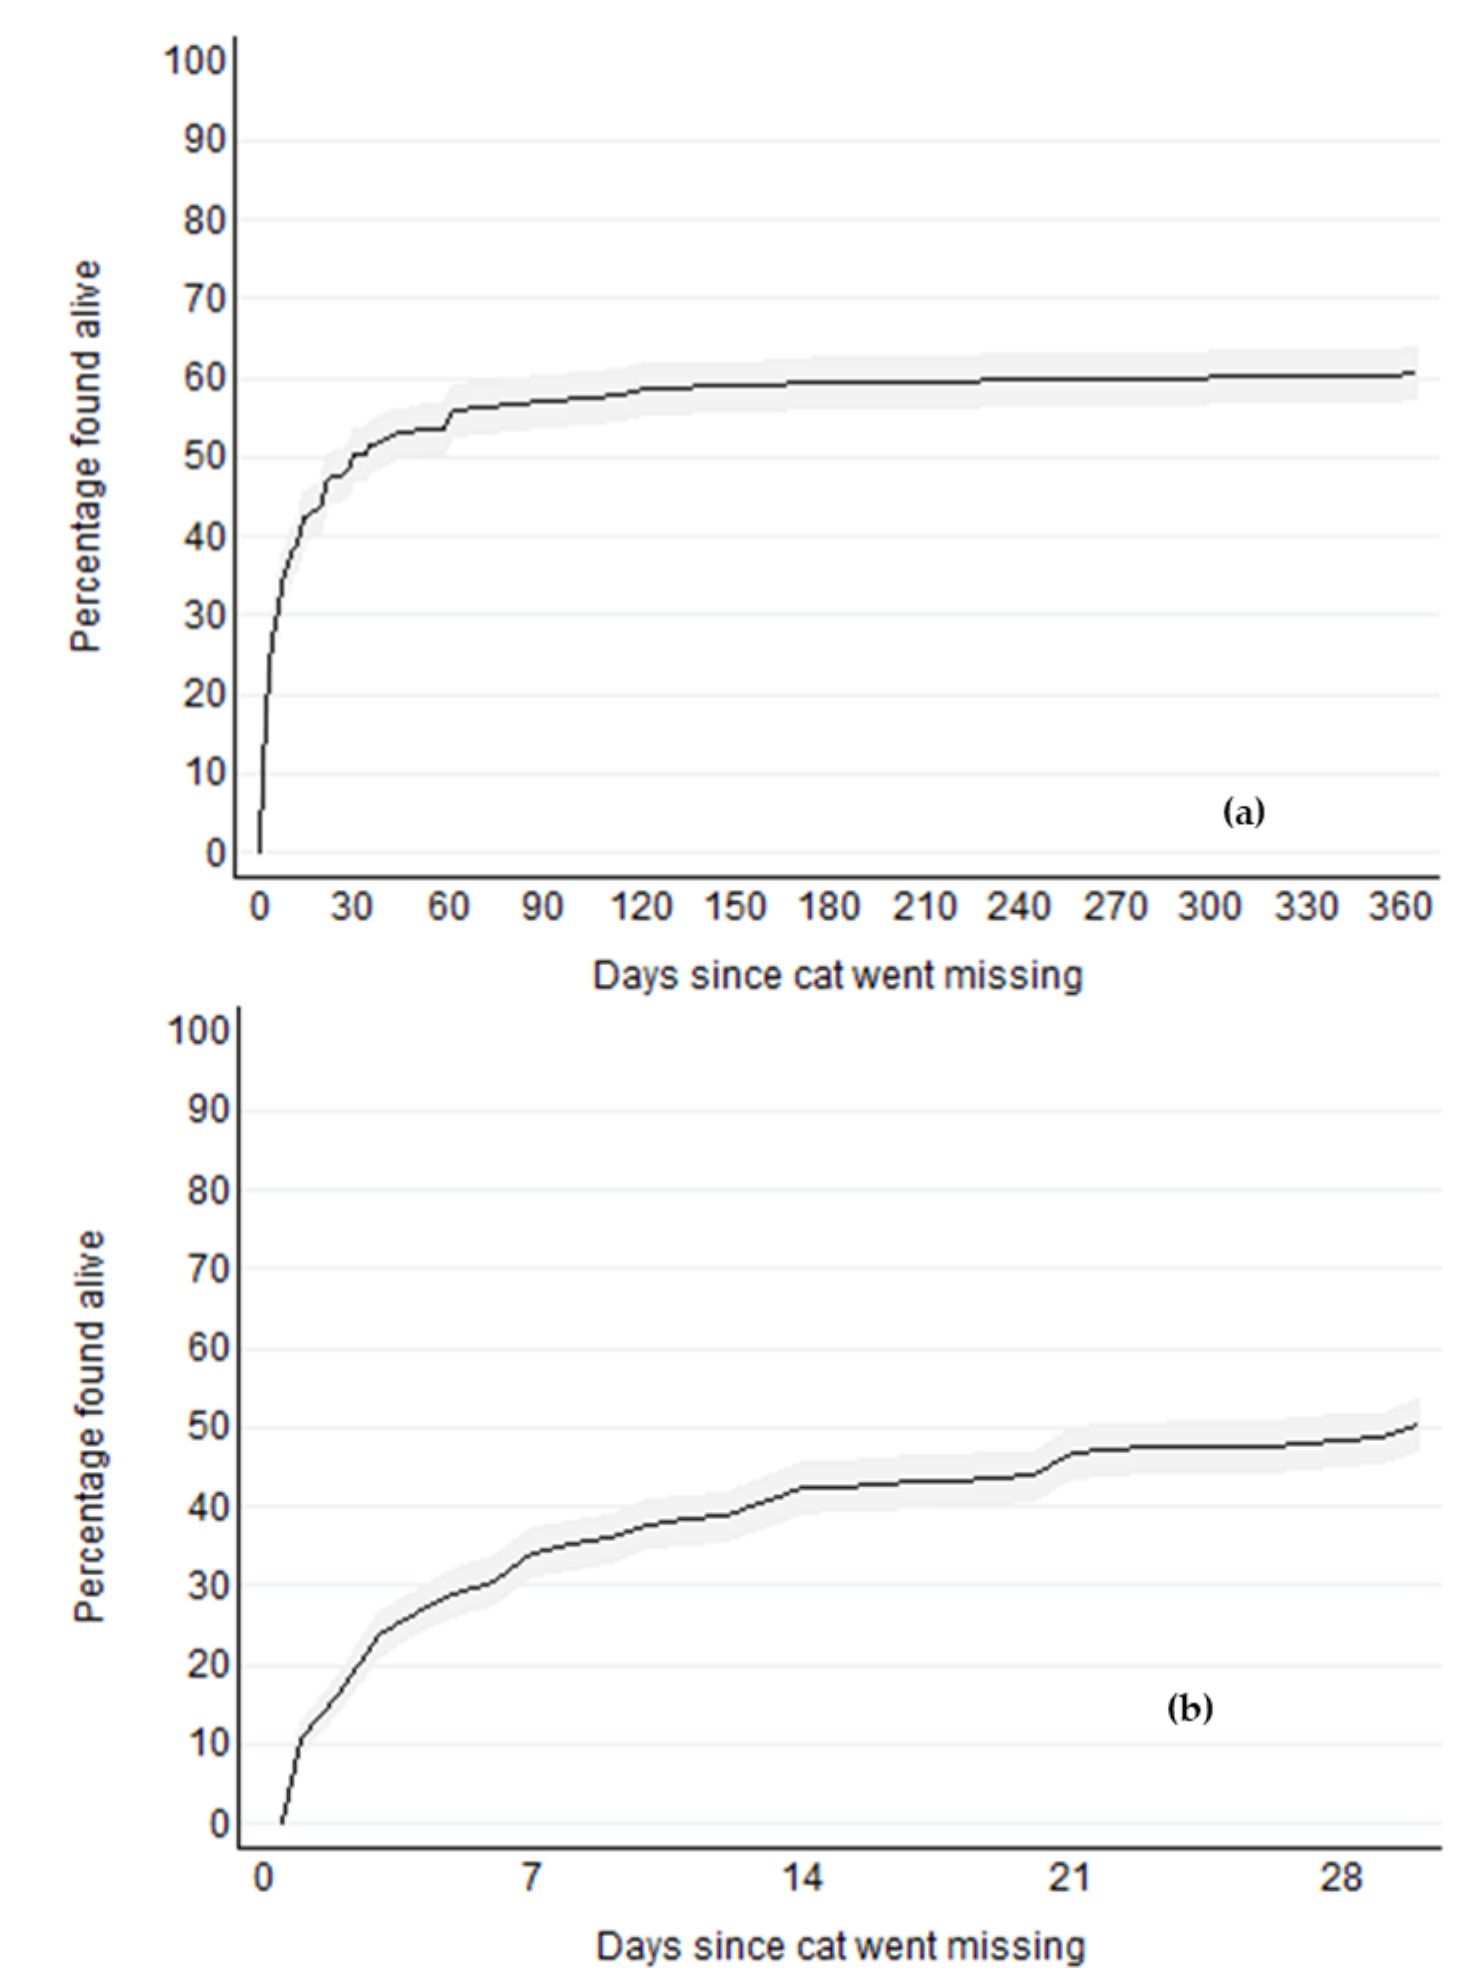
\includegraphics[width=0.44\textwidth]{imagens/01_pesquisa/figura01_curva_recuperacao_tempo.png}
    \fonte{Adaptado de Huang et al. (2018, p. 9)}
\end{figure}

Conforme evidencia a Figura~\ref{fig:curva_recuperacao_tempo}, aproximadamente 34\% dos gatos resgatados com vida foram encontrados logo na primeira semana de buscas e 50\% nos primeiros trinta dias, observando-se pouca evolução no índice de recuperação após sessenta dias. Esse comportamento ressalta a importância de ferramentas que permitam a emissão rápida de alertas e a circulação imediata de informações para a comunidade, de modo a maximizar as chances de localização dentro dessa janela temporal decisiva.

Além do tempo de resposta, o sucesso da recuperação relaciona-se diretamente à proximidade geográfica do local de fuga. Huang et al. (2018) constataram que metade dos gatos foi localizada a até 50 metros e 75\% em um raio de até 500 metros do ponto de desaparecimento, podendo atingir até cerca de 1,6~km naqueles habituados ao ambiente externo. O estudo revelou ainda que menos de 2\% dos gatos reencontrados vivos estavam em abrigos municipais ou centros de zoonoses. O êxito decorreu majoritariamente de buscas ativas no entorno imediato, da cooperação de vizinhos para averiguar pátios e garagens e da utilização de avisos e cartazes físicos e digitais. Esses dados indicam que as estratégias mais eficazes concentram-se na vizinhança e reforçam a necessidade de articulação colaborativa local.

Entre as formas de divulgar a perda de um animal estão o contato com vizinhos e clínicas veterinárias, a distribuição de cartazes e as publicações em redes sociais e grupos de mensagens. Na pesquisa de campo deste trabalho, os participantes também indicaram o uso desses diferentes canais, conforme detalhado no Capítulo 3.

Quando o caso é divulgado em diferentes canais, as informações e atualizações podem ficar distribuídas entre páginas, grupos e conversas. Por exemplo, uma atualização sobre o telefone de contato ou sobre um novo local onde o animal foi visto pode aparecer em apenas um canal. Essa possibilidade pode dificultar o acompanhamento da busca e evidencia a importância de manter as informações organizadas. Essa questão também foi investigada na pesquisa de campo apresentada no Capítulo 3.

Apesar dessas dificuldades, a divulgação permite que outras pessoas participem da busca. Um morador pode reconhecer o animal pela foto e informar onde o viu; outra pessoa pode acrescentar um novo relato mais tarde, em outro ponto da região. Quando reunidas, as descrições, os horários e os locais ajudam a compor um histórico mais claro da procura.

Essa dinâmica se relaciona aos sistemas colaborativos, que apoiam a interação entre pessoas envolvidas em uma atividade comum. Fuks et al. (2011) explicam a colaboração por meio de três aspectos relacionados: comunicação, coordenação e cooperação. A comunicação envolve a troca de informações entre os participantes. A coordenação organiza essas interações e contribuições em torno da atividade compartilhada. A cooperação ocorre quando as pessoas atuam sobre informações e recursos comuns para alcançar um objetivo. Na busca por animais, esses aspectos aparecem quando os participantes divulgam informações sobre o animal, acrescentam relatos de avistamento e consultam os dados reunidos em uma publicação. Um sistema colaborativo pode apoiar esse processo ao vincular as contribuições à publicação correspondente e facilitar o acompanhamento das atualizações, sem garantir o reencontro do animal.

No contexto brasileiro, soluções computacionais para apoiar essas buscas também têm sido propostas. Souza et al. (2022), por exemplo, apresentam o FugaPet-Rotas, um algoritmo que recomenda rotas para orientar a procura por animais desaparecidos. Na busca exploratória realizada para este trabalho (Capítulo 3), não foram identificados, entre as fontes consultadas, estudos que reunissem em um mesmo aplicativo a organização geográfica das publicações, o registro de avistamentos vinculados a cada caso e a comunicação privada entre os participantes; essa constatação, contudo, limita-se às bases e aos termos pesquisados.

O Capítulo 3 apresenta a pesquisa de campo e a análise de sistemas similares utilizadas para identificar as necessidades relacionadas à divulgação e ao acompanhamento das buscas.
